%%%--------------------------------%%%
%%% UC7
%%%--------------------------------%%%

\newpage
% UC7 ====================================================
\subsubsection{Use Case Specification: \ac{UC}7 Risk Monitoring}
\label{sec:domainBbh}

\paragraph*{Description}\mbox{}\\
This \ac{UC} deals with the monitoring of risks. It enables to remind the project team and its members to treat the defined risks.

\paragraph*{Screenshots}\mbox{}\\
tbd: Insert screenshots and shortly explain what can be seen
\begin{figure}[h] 
	\centering
	
\includegraphics[width=0.1\textwidth]{Content/Domain/placeholder.png}
	\caption{Use Case X: Detail}
	\label{fig:label7}
\end{figure}

\paragraph*{Basic Flow} \mbox{}\\
\noindent
The risk's response defines if the defined action is done one-time or on a regular basis. 

\noindent
One-time:
\begin{itemize}
	\vspace{-3mm}
	\setlength\itemsep{-1em}
	
	\item When adding a response to a risk which is only processed one time the user can set a fixed date due to the response should be done.
	\item Before the deadline the person in charge is notified. "Have you already done <the response> (Yes | No)".
\end{itemize}

\noindent
Regular basis:
\begin{itemize}
	\vspace{-3mm}
	\setlength\itemsep{-1em}
	
	\item When adding a response to a risk which is processed on a regular basis the user can set an interval in which the response should be done.
	\item The person in charge is notified in this interval. "Have you already done <the response> (Yes | No)".
\end{itemize}


\subparagraph{Activity Diagram}\mbox{}\\
\begin{figure}[H]
	\centering
	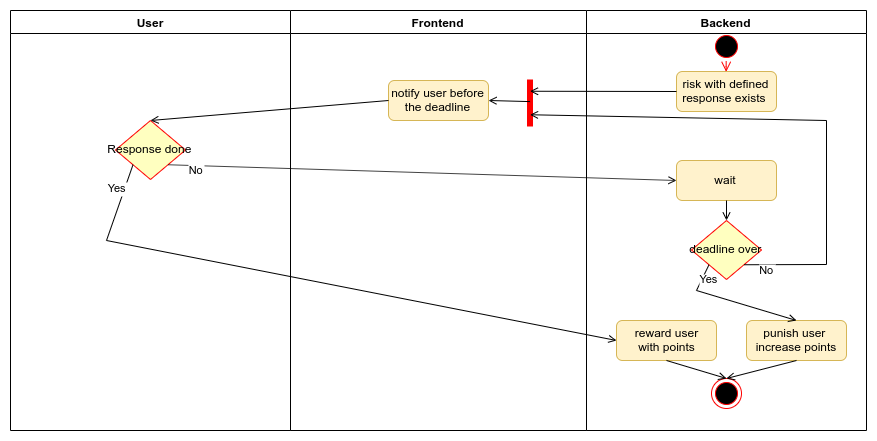
\includegraphics[width=1.0\textwidth]{Content/Domain/UC7RiskMonitoring.png}
	\caption{Activity Diagram \ac{UC}7 Risk Monitoring}
	\label{fig:label77}
\end{figure}

\paragraph*{Alternative Flows}\mbox{}\\
N/A

\paragraph*{Special Requirements and Preconditions}\mbox{}\\
The preconditions for this use case are:
\begin{enumerate}
	\vspace{-3mm}
	\setlength\itemsep{-1em}
	
	\item A project exists.
	\item The user is member of the project.
	\item The user is person in charge of a risk.
\end{enumerate}

\paragraph*{Postconditions and Persistance}\mbox{}\\
The postconditions for this use case are:
\begin{enumerate}
	\vspace{-3mm}
	\setlength\itemsep{-1em}
	
	\item Best case: The risk's response was done and the user in charge is rewarded.
	\item Undesired case: The risk's response was not done due to the deadline and the user in charge is punished.
\end{enumerate}